\chapter{Application 1: Multilingual Geocoder based on labels using Time and Language Features}\label{chap:ch6}

\section{Introduction}
As has been shown in Chapter 2, it is inherently difficult to build a universal geocoding solution that can handle various languages and their associated alphabets, popular slang, and purposely ambiguous phrases on Twitter. In a step towards a universal geocoding solution, Chapter 5 showed that time-based features could be used for identifying whether the user group is from a particular timezone. A timezone spans a large geographic area, but the language features can constrain the set of possible countries. In this chapter, the proposed approach is illustrated by categorizing 320K Twitter influencers. High confidence influencer predictions are used as training data for an improved geocoder. This geocoder automatically learns popular ways that Twitter users refer to locations within the country and can handle foreign alphabets.

\section{Influencers-Dataset}

In this dataset, user groups are binned by the influencer they follow. The influencers for the dataset were chosen from the special Twitter \emph{@verified}. It tracks all influencers that have passed an internal Twitter check (after Twitter performs a special check the influencer is identified via a special blue badge). In this dataset, collected in the spring of 2019, there are 320,166 influencers. Due to Twitter API limits, for each influencer only a single API call was made which returned at most 5000 followers.

The ground truth consists of the country associated with the self-reported location reported by the influencer. It is checked whether this country can be used as a label, based on whether this country matches (i) the most frequent country from self-reported locations of followers and (ii) whether it is contained within the set of countries that would be predicted using followers' time and language features. It is shown that time and language features can be used to improve the precision of the country labels. The country label and the associated influencer's followers' self-reported locations are used for training and illustrating a multilingual geocoder. 

\section{Incorporating Language} 
We utilize language to further improve the performance of the time-based classifier proposed in section 5.3. Given a time distribution associated with a user group we can compute $UTC^P$ (equation (5.2)). Let $U_1$ equal the set of countries whose cities have a time zone that observes UTC offset in the range $[UTC^P-t_1 , UTC^P + t_1]$, where $t_1$ is a preselected threshold.  For example,  the set of countries [TLS, PLW, JPN, MNP, FSM, GUM, IDN, AUS, PRK, RUS, KOR, PNG], correspond to UTC range $\in$ [8, 10].

Our next step is to incorporate language information to constrain the set of possible countries for the selected UTC offset range. Initially, the CIA World Factbook was utilized for this purpose. But for some countries, the languages from CIA World Factbook did not align with the languages used on Twitter. For example, English is the most popular language in India for communication, but it does not make it into popularly spoken languages (instead Hindi, Bengali, and others are listed).

We utilized language preferences, a user-selected option, which is available for more than 99\% of collected users on Twitter. In our dataset, there are 76 unique language codes associated with 143 countries, each language was used by at least 100 users, collected over 373 million user profiles. 

Given a user group, the users' language preferences are used to generate a language distribution, i.e., we calculate:

\[ g_G(\ell) = \frac{\text{\# of users of language } \ell \text{ in } G}{|G|}\]
for all 76 languages. The language distribution for all countries was also calculated, i.e.,

\[ h_c(\ell) = \frac{\text{\# of users of language } \ell \text{ in country } c}{\text{\# of all users in country } c}\]
for all 143 countries.

Using cosine similarity  $g_G(\ell)$ is compared with  $h_c(\ell)$ for all 143 countries. Let $U_2$ be the set of countries whose language distributions have a similarity score greater than threshold $t_2$. Finally, let $U_3 = U_1 \cap U_2$ that is, $U_3$ equals the set of countries common to both sets $U_1$ and $U_2$.

Table \ref{table_4app} shows how the language distributions helps narrow down the list of possible countries for different thresholds $t_2$. Recall that for each user group in the UTC offset dataset its location and therefore its country is known. For each user, if this country is in set $U_i$ then the prediction is marked correct, incorrect otherwise. In Table \ref{table_4app} the first three columns are the median number of countries associated with $U_1$, $U_2$, and $U_3$. 

\begin{table}[htbp]
\small
\caption[Constrain set of possible countries via language]{Language helps constrain the set of possible countries from UTC while improving precision for higher cosine similarity, $t_2$}
\label{table_4app}
\centering
\begin{tabular}{|c|c|c|c|c|c|}
\hline
\bfseries U\textsubscript{1} & \bfseries U\textsubscript{2} & \bfseries U\textsubscript{3} & \bfseries P & \bfseries R & \bfseries t\textsubscript{2} \\
\hline
19 & 143 & 17 & 89.02 & 100.00 & 0.05 \\
\hline
19 & 140 & 17 & 89.14 & 99.87 & 0.15 \\
\hline
19 & 127 & 12 & 89.54 & 99.42 & 0.25 \\
\hline
19 & 115 & 8 & 89.75 & 99.18 & 0.35 \\
\hline
19 & 108 & 7 & 90.07 & 98.80 & 0.45 \\
\hline
19 & 102 & 7 & 90.23 & 98.58 & 0.55 \\
\hline
19 & 99 & 6 & 90.32 & 98.38 & 0.65 \\
\hline
19 & 91 & 6 & 90.27 & 98.23 & 0.75 \\
\hline
19 & 83 & 5 & 90.26 & 97.84 & 0.85 \\
\hline
19 & 70 & 4 & 90.34 & 96.01 & 0.95 \\
\hline
\end{tabular}
\end{table}

It can be seen that our final prediction, identified by the set $U_3$, has good accuracy and a much smaller set of possible countries then initial $U_1$. From table, values from 0.85 to 0.95 work well for $t_2$.

\section{Illustration over Influencers-Dataset}
The prediction methods, discussed in previous sections, are shown in a pipeline in Fig. \ref{fig_6app}. As an application, the pipeline is applied over Influencers-Dataset. The goal is to identify geo-influencers and accurately associate them with the country that most of their followers are from. We are interested in high confidence influencer predictions because these in turn can be used as training data for a multilingual geocoder that will be presented in the following section. 

\begin{figure}[h!]
\centering
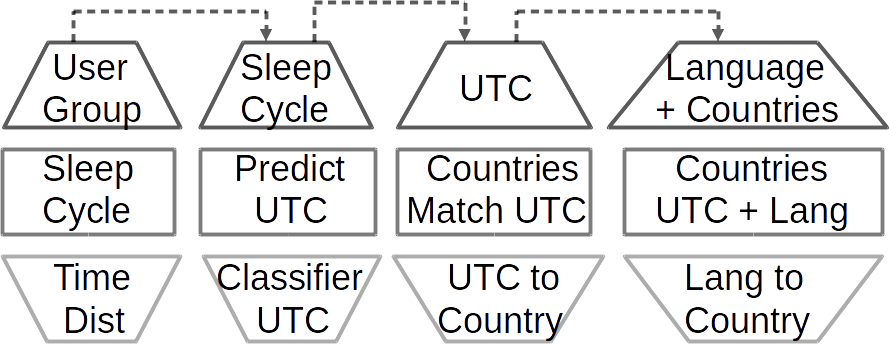
\includegraphics[width=4.5in]{FigA882}
\caption[Pipeline for predicting region of the world]{Pipeline for predicting region of the world using time and language features. The top layer shows input, the middle layer output, and the bottom layer the name of the process. Each step sends its output as input to the next step.}
\label{fig_6app}
\end{figure}

One data point is the influencer's self-reported location. Another data point is the ratio of followers' self-reported locations belonging to a particular country. The expectation is that for geo-influencers the country associated with the self-reported location will match the most frequent country from influencer's followers. Self-reported locations that match a known GeoNames entry are utilized as described in section 5.3.1.

A problem with self-reported location information from followers is that the labeled location focuses on the Latin alphabet with foreign city names appearing as they would be referred to by an English speaker (Moscow instead of Moskva in Cyrillic). Therefore, English-speaking users are incorporated more often than non-English speakers. Using the following steps we aim to test the different stages from Fig. \ref{fig_6app} to help with this imperfect baseline:

\begin{enumerate}
\item Step 1a (S1a) -- Get rid of influencers whose followers' time distribution does not exhibit a U-shaped parabola.
\item Step 1b (S1b) --  Get rid of those influencers which are classified as global.
\item Step 2 (S2\_$t_1$) -- $UTC^P$ computed and used to obtain the set of possible countries $U_1$.
\item Step 3 (S3\_$t_2$) -- Reduce  the set $U_1$ to set $U_3$ by constraining to countries that have cosine similarity above $t_2$.
\end{enumerate}

Steps S1a and S1b should reduce the dataset to focus primarily on geo-influencers whose followers are concentrated in a single time zone. Steps S2\_$t_1$ and S3\_$t_2$ help identify and correct instances where the baseline is making poor predictions that do not match using countries based on time and time+language features, respectively. If the top-ranked country from the baseline is within the set of countries it is returned as a prediction otherwise the second top country is used and so on. 

There were 100,712 influencers with a self-reported location that could be resolved using GeoNames. The country that the influencer associates themselves with is used as ground truth. For example, \emph{@BBCNews} has a self-reported location `London' which is associated with GBR using GeoNames. 
Ordering by the most frequent country from followers' self-reported locations, the top five countries and associated percent of self-reported locations are USA: 28.15\%, NGA: 10\%, IND: 6.3\%:, GBR: 5.92\%, and KEN: 4.81\%. Thus, USA is the top prediction used in baseline, but this does not match the set of possible countries from S2\_$t_1$ and so NGA is used as it is the second best prediction; NGA has the same UTC as GBR and is thus within the set of possible countries using time features. Language features from S3\_$t_2$ can further constrain the prediction to the expected result, GBR.

In the above, we have described a procedure that results in a set of possible countries making up $U_3$. We also consider a point estimate prediction where a single country with the best cosine similarity is returned for a narrow UTC range $t_1=0.25$ (this point estimate is denoted as S3\_Point in Table \ref{table_5app}).

Table \ref{table_5app} shows how the baseline is constrained using each step of the pipeline. The second column shows precision across all influencers (100,712) and the fourth column shows precision across influencers not associated with the USA (37,908).

\begin{table}[htbp]
\small
\caption{Different Stages of Pipeline Improve Baseline Precision}
\label{table_5app}
\centering
\begin{tabular}{|c|c|c|c|c|}
\hline
& \bfseries All P & \bfseries Count & \bfseries Foreign P & \bfseries Count\\
\hline
Baseline & 86.34 & 100708 & 65.71 & 37904 \\
\hline
S1a & 86.23 & 95500 & 65.61 & 36087 \\
\hline
S1b & 89.98 & 71643 & 76.97 & 28725 \\
\hline
S2\_1 & 90.23 & 70544 & 77.39 & 28018 \\
\hline
S2\_0.5 & 90.95 & 65708 & 78.98 & 25845 \\
\hline
S2\_0.25 & 92.23 & 60387 & 79.43 & 20753 \\
\hline
S2\_1+S3\_0.95 & 91.49 & 64940 & 78.15 & 23315 \\
\hline
S2\_0.5+S3\_0.95 & 92.78 & 57584 & 80.86 & 19721 \\
\hline
S2\_0.25+S3\_0.95 & 94.54 & 50978 & 80.94 & 13395 \\
\hline
S2\_0.25+S3\_Point & 97.2 & 35518 & 86.59 & 6587 \\
\hline
\end{tabular}
\end{table}

Table \ref{table_5app} illustrates that as time and language constraints are added the precision improves. Removing influencers that don't pass the sleep cycle test surprisingly doesn't help (row S1a), but getting rid of influencers with noisy PST predictions (row S1b) results in a big jump in precision.% (both measures are related to focusing on geo-influencers which are expected to have a strong follower concentration in a single geographic area). 
UTC offset information further constrains the baseline (rows S2\_$t_1$). 
%{The smaller the $t_1$ the smaller is the geographic area that needs to be matched using baseline. }
The highest precision is achieved when both UTC and language information are used. 

\section{Training Geocoder with Support for Foreign Languages}

As already noted, the issue with the baseline Geocoder was that it handles only English based locations that have a match to GeoNames. Our proposed approach is to use the high confidence influencer predictions from the previous section as training data for an improved geocoder. This geocoder will automatically learn common ways persons refer to locations in their native tongue. 

This new geocoder is based on a TF-IDF model, where the country is the document and the terms are the self-reported locations of the influencer's followers. It is possible to apply this model because if the influencer and their followers belong to the same country, then the followers' locations will capture common ways persons refer to locations within that country. TF-IDF vectors are generated using the Gensim package in Python\footnote{https://radimrehurek.com/gensim/}. 

\iffalse
From equation \eqref{eq122}, the weights of TF-IDF are based on the frequency of term $i$ in document $j$ times log inverse ratio of total documents with the term over total $D$ documents. 
\begin{equation}
TF-IDF_{i,j} = frequency_{i,j}*log_2\frac{D}{doc_{freq_i}}\label{eq122}
\end{equation}
\fi

Focusing on the top $K$ TF-IDF features per country it is possible to verify that the model is generating reasonable vectors. Fig. \ref{fig_7app} shows the top three features for several countries. These strings capture typical ways persons refer to locations within that country which can serve as useful features for geocoding type classifiers. The model also helps confirm that the countries, with which the influencer's followers were associated with, are indeed relevant.

\begin{figure}[!t]
\centering
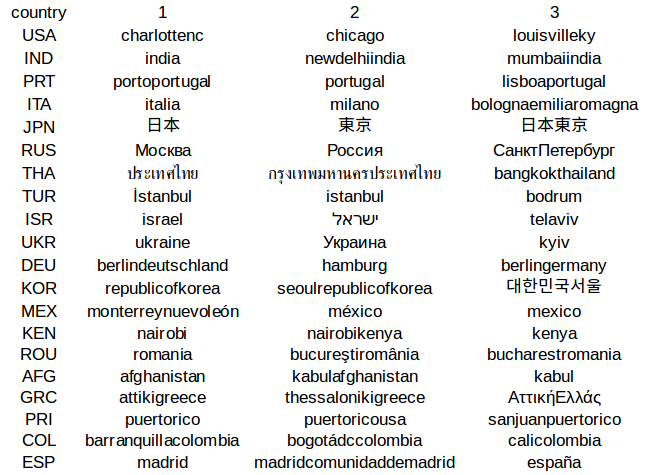
\includegraphics[width=4.7in]{FigA7}
\caption[Features from Multilingual TF-IDF Geocoder]{Top three TF-IDF location features automatically learned from country documents. The benefit of this model is that it learns popular ways of referring to the country's locations in different languages and will include common phrases, abbreviations, and so on.}
\label{fig_7app}
\end{figure}

Given a new influencer, the self-reported locations associated with the influencer's followers form a new document. A TF-IDF vector is built using self-reported location frequencies and the IDF component previously computed over the corpus of $D$ documents. Cosine similarity is then used to return the country vector that is closest to the TF-IDF vector. Because the TF-IDF vectors may be very large, we recommend utilizing Latent Semantic Analysis (LSA) to reduce dimensionality to at most 500 terms (from literature 50-500 is recommended as a standard [\ref{appendix:6b.17}]). Fig. \ref{fig_78app} highlights the overall approach. 

\begin{figure}[!t]
\centering
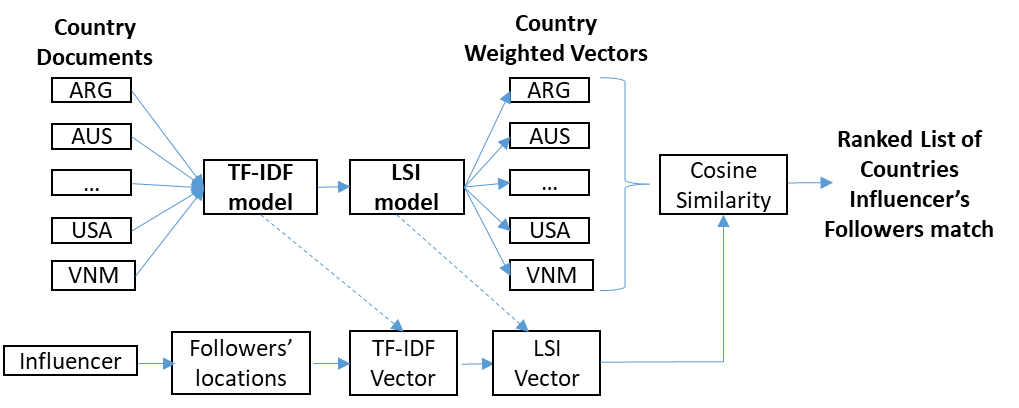
\includegraphics[width=5.7in]{FigA88}
\caption[Training TF-IDF Geocoder]{The process by which TF-IDF model is learned from geo-influencers associated with a country and used for predicting other geo-influencers.}
\label{fig_78app}
\end{figure}

In Table \ref{table_6app}, the performance of the TF-IDF model is shown against the baseline from the previous section. TF-IDF model has a higher precision than original baseline with a clear jump in precision for foreign countries. This improved geocoder can be used to generate labels across additional influencers (that could not be predicted using the original baseline). The additional labels can be verified using time and language features and the TF-IDF model can be further improved. The process can repeat until the process converges, that is, when the TF-IDF model no longer improves.

\begin{table}[htbp]
\small
\caption{TF-IDF model performance for Different Stages of Pipeline}
\label{table_6app}
\centering
\begin{tabular}{|c|c|c|c|c|}
\hline
& \bfseries All P & \bfseries Count & \bfseries Foreign P & \bfseries Count\\
\hline
Baseline & 86.34 & 100708 & 65.71 & 37904 \\
\hline
TF-IDF model & 88.44 & 100711 & 81.75 & 37907 \\
\hline
\end{tabular}
\end{table}

\section{Conclusions}
This chapter showed an application by which the geographic region can be labeled using only time and language features. The benefit of our approach is that these time and language features are universal and can be used across the whole Twittersphere. The labels have been used to train a high-level geocoder that has multilingual support. The benefits are that the common ways that Twitter users report their locations are captured by this geocoder. The drawback to our method is that it works at a high level for predicting regions of the world at the country level or larger. We envision that the features proposed will be utilized for augmenting with other features as part of information fusion.